\documentclass[11pt,a4paper]{article}
\usepackage[margin=1in]{geometry}
\usepackage{times}
\usepackage{amsmath,amssymb}
\usepackage{hyperref}
\usepackage{enumitem}
\usepackage{titlesec}
\usepackage{parskip}
\usepackage{tikz}
\usetikzlibrary{arrows.meta,positioning,shapes.geometric}
\usepackage{framed}
\usepackage{xcolor}

\hypersetup{colorlinks=true, linkcolor=blue, citecolor=blue, urlcolor=blue}
\titlespacing*{\section}{0pt}{12pt}{6pt}
\titlespacing*{\subsection}{0pt}{10pt}{4pt}
\definecolor{noteback}{RGB}{240,244,255}

\title{\vspace{-1.5cm}\textbf{Physical Attacks on Lattice-Based\\ Post-Quantum Cryptography: A Survey,\\ Replication, and Improvement Study}\\[4pt]
\large A Draft Research Proposal --- Beginner-Friendly Version}
\author{}
\date{}

\begin{document}
\maketitle
\vspace{-1.0cm}

\begin{framed}
\small\noindent\textbf{A note before you start reading.} This document assumes no prior background in lattice-based cryptography. Every technical term is explained in plain language the first time it appears, and a full glossary is at the end (Section~9) for quick lookup. If a sentence still feels dense, it's worth flagging in our lecture sessions --- that's exactly the kind of thing we should slow down on together.
\end{framed}

\section*{1. Background: Why This Topic, in Plain Words}

\subsection*{1.1 The problem: computers are about to get much more powerful}
Every time you send a message over the internet, use online banking, or connect to Wi-Fi, some form of \textbf{cryptography} (mathematics-based secret-keeping) is protecting your data. Most of the cryptography in use today (called RSA and elliptic-curve cryptography) is secure because certain math problems are extremely hard for ordinary computers to solve --- it would take longer than the age of the universe to break them by brute force. The catch: a \textbf{quantum computer}, a fundamentally different type of computer that is still being built by several companies and governments, is expected to be able to solve those particular math problems quickly once it is powerful enough. So the whole world needs to move to cryptography based on \emph{different} math problems that even a quantum computer cannot solve efficiently. This global effort is called \textbf{post-quantum cryptography (PQC)}.

The organization leading this transition is the \textbf{National Institute of Standards and Technology (NIST)}, a US government agency that runs open competitions to pick the best new algorithms and turns them into official standards that the whole world can adopt. After several years of public competition, NIST selected a small number of winning algorithms. Most of them belong to a family called \textbf{lattice-based cryptography}, which is the subject of this thesis.

\subsection*{1.2 What is a ``lattice''?}
Imagine an infinite grid of evenly-spaced dots stretching in every direction --- like graph paper, but the dots can be in many more than two dimensions (lattice-based cryptography typically uses hundreds of dimensions, which is impossible to draw but works the same way mathematically). This grid of dots is called a \textbf{lattice}. Figure~\ref{fig:lattice} shows a simplified 2-dimensional version.

\begin{figure}[h]
\centering
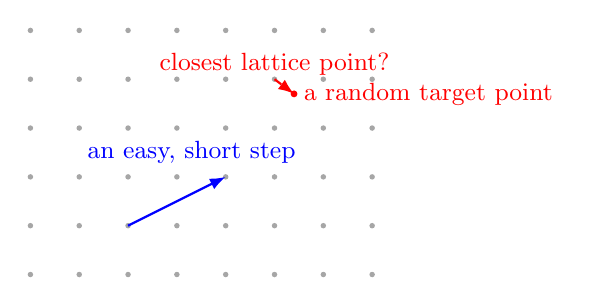
\begin{tikzpicture}[scale=0.62]
  \foreach \x in {0,...,7}
    \foreach \y in {0,...,5}
      \fill[gray!70] (\x,\y) circle (1.6pt);
  \draw[-{Latex[length=2mm]}, thick, blue] (2,1) -- (4,2);
  \node[blue, font=\small] at (3.3,2.5) {an easy, short step};
  \fill[red] (5.4,3.7) circle (2pt);
  \node[red, font=\small, right] at (5.4,3.7) {a random target point};
  \draw[-{Latex[length=2mm]}, thick, red, dashed] (5,4) -- (5.4,3.7);
  \node[red, font=\small] at (5,4.3) {closest lattice point?};
\end{tikzpicture}
\caption{A tiny, simplified 2-D lattice (real schemes use hundreds of dimensions). Taking a few short, simple steps between dots is easy. But given a \emph{random} point that is not exactly on the grid, figuring out which dot is closest to it --- or reconstructing which combination of short steps could reach near it --- becomes extremely hard once the grid has enough dimensions.}
\label{fig:lattice}
\end{figure}

Two things make lattices useful for cryptography: (1) it is easy to \emph{build} a lattice and move around on it if you know a special, secret ``short path'' description of it (this is used as the private/secret key); (2) it is believed to be extremely hard --- even for a quantum computer --- to figure out that short-path description, or to answer certain questions about the lattice (like ``what is the closest grid point to this random spot?''), if you only see the lattice described in an ordinary, ``scrambled'' way (this becomes the public key, and the hardness is what keeps the secret safe). The specific hard question used by the algorithms in this thesis is called \textbf{Learning With Errors (LWE)}: roughly, the secret is hidden inside a bunch of equations that have a small amount of random ``noise'' mixed in, on purpose, and recovering the secret from the noisy equations is the hard part \cite{menezes2026gentle}.

\subsection*{1.3 The specific algorithms we care about}
NIST's selected lattice-based algorithms include:
\begin{itemize}[leftmargin=*]
  \item \textbf{ML-KEM (nicknamed Kyber):} used to let two parties agree on a shared secret key over an insecure channel (a ``key encapsulation mechanism'', or KEM) --- this is the lattice-based replacement for how your browser currently sets up an encrypted connection.
  \item \textbf{ML-DSA (nicknamed Dilithium)} and \textbf{Falcon:} used to create digital signatures --- the lattice-based replacement for how software updates, documents, or transactions are digitally ``signed'' to prove who created them and that they haven't been tampered with.
\end{itemize}
These are not experimental anymore --- they are official standards now being rolled out in web browsers, VPNs, smartcards, hardware security modules, and embedded devices. That real-world rollout is exactly why studying their security in practice, not just on paper, matters right now.

\subsection*{1.4 Two very different ways to ``attack'' a cryptographic scheme}
There are two largely separate research traditions for trying to break a scheme like Kyber or Dilithium, and it's worth being clear about the difference from the start, because this thesis focuses on only one of them.

\textbf{(a) Mathematical / algorithmic attacks.} These try to solve the underlying hard lattice problem directly --- essentially, finding a clever algorithm that finds the closest grid point (or the secret short path) faster than anyone previously knew how to. This is classical, ``pen and paper'' cryptanalysis; researchers who do this need deep, specialized background in lattice algorithms, and progress tends to be slow and incremental. \textbf{This is not what this thesis is about}, but it is useful context: it's the reason NIST believes these schemes are safe against quantum computers in the first place \cite{ducas2025predicting}.

\textbf{(b) Implementation (physical) attacks --- the focus of this thesis.} These attacks completely ignore the underlying math problem. Instead, they exploit \emph{how} a real chip or program executes the algorithm. A useful analogy: imagine a bank vault with an unbreakable combination lock (the math is secure), but the safecracker doesn't need to break the lock at all --- they can listen to the faint clicks the dial makes as the legitimate owner turns it, and work out the combination that way. Two common physical-attack families:

\begin{itemize}[leftmargin=*]
  \item \textbf{Side-channel attacks (SCA):} while a chip performs a computation, it consumes electrical power, gives off electromagnetic radiation, and takes a certain amount of time --- and all of these physically measurable signals can depend, in subtle ways, on the secret key being used, even though the program's official output does not reveal it. An SCA measures these signals (for example, with a small probe placed near the chip while it runs, connected to an oscilloscope --- a device that records how a signal changes over time) and uses statistics to guess the secret key, a small piece at a time. Figure~\ref{fig:scapipeline} sketches this process.
  \item \textbf{Fault-injection attacks (FIA):} instead of just \emph{watching}, the attacker deliberately \emph{disturbs} the device --- for example, with a brief voltage spike, a disrupted clock signal, or a laser or electromagnetic pulse --- at a precisely timed moment, to force the chip to make a computational mistake. The attacker then studies the incorrect (``faulty'') output the device produces and works backward to recover the secret key.
\end{itemize}

\begin{figure}[h]
\centering
\resizebox{\textwidth}{!}{%
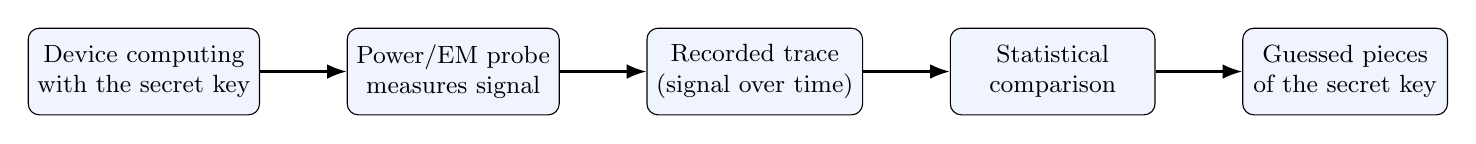
\begin{tikzpicture}[
  box/.style={draw, rounded corners, align=center, minimum width=2.6cm, minimum height=1.1cm, font=\small, fill=noteback},
  arr/.style={-{Latex[length=2.5mm]}, thick}
]
  \node[box] (dev) {Device computing\\ with the secret key};
  \node[box, right=1.1cm of dev] (probe) {Power/EM probe\\ measures signal};
  \node[box, right=1.1cm of probe] (trace) {Recorded trace\\ (signal over time)};
  \node[box, right=1.1cm of trace] (stats) {Statistical\\ comparison};
  \node[box, right=1.1cm of stats] (key) {Guessed pieces\\ of the secret key};
  \draw[arr] (dev) -- (probe);
  \draw[arr] (probe) -- (trace);
  \draw[arr] (trace) -- (stats);
  \draw[arr] (stats) -- (key);
\end{tikzpicture}%
}
\caption{A simplified side-channel attack pipeline. No step here involves solving the underlying lattice math problem.}
\label{fig:scapipeline}
\end{figure}

Why this matters: a scheme can be mathematically flawless --- provably secure against every known attack in family (a) --- and still be broken in minutes, using cheap and widely available equipment, because of a weakness in family (b). This has now been demonstrated, in published research, against essentially every major lattice-based NIST algorithm (Kyber, Dilithium, Falcon, and the related NTRU scheme). That combination --- rock-solid math, but leaky real-world implementations --- is precisely the gap this thesis explores.

\section*{2. Related Work (What Has Already Been Done)}

Physical attacks on lattice-based cryptography have become a large, active research area over the last several years. Below, each result is first described in plain terms, then linked to its source.

\begin{itemize}[leftmargin=*]
  \item \textbf{Kyber (ML-KEM).} Researchers combined a power-measurement technique with a mathematical clean-up step to extract the \emph{entire} secret key of Kyber running on a real, low-power chip, using only about 15 short power measurements and roughly 10 minutes of computer time afterward \cite{wang2024twostep}. In plain terms: with cheap equipment and a short lab session, the ``unbreakable'' key came out anyway --- not because the math was wrong, but because the chip leaked information while using it. Separately, a common performance shortcut used inside many lattice implementations, called \emph{central reduction} (a way of keeping numbers small and computations fast), was shown to accidentally leak the plus/minus sign of secret intermediate values through power consumption, which cut the number of measurements needed to break even \emph{protected} implementations by roughly 100$\times$ \cite{exploitcentralreduction2024}.
  \item \textbf{Dilithium (ML-DSA).} A technique called a ``signature correction'' attack exploits small amounts of information that leak while the device produces a digital signature; combined with lattice math and side-channel ``hints,'' this recovers the secret signing key using fewer measurements than previously thought possible \cite{signaturecorrection2022, dachmansoled2020lwesideinfo}. Separately, researchers showed that when a signature scheme always produces the exact same signature for the exact same message (called being \emph{deterministic}), this predictability can be combined with a deliberately injected computational fault to recover the secret key --- demonstrated directly on real embedded-device implementations of NIST candidates including Dilithium \cite{ravi2019exploitingdeterminism}.
  \item \textbf{Falcon.} Falcon is unusual among these schemes because part of its computation uses \emph{floating-point} arithmetic (numbers with decimal points, like $3.14159$, as opposed to the whole numbers most cryptography uses) and a specific random-sampling step called \emph{discrete Gaussian sampling} (drawing random numbers so that values near zero come up more often than large ones, following a bell-curve-like pattern). Both of these have repeatedly proven hard to protect. ``Falcon Down'' showed that a side-channel attack could recover Falcon's secret key by targeting this sampling step \cite{karabulut2021falcondown}; a more recent attack recovers the \emph{entire} key from a \emph{single} power measurement by exploiting one specific low-level operation (a ``shift'' instruction) used during key creation \cite{singletracefalcon2025}; and a fault attack has been shown to work against the deterministic version of Falcon using only one well-timed fault \cite{bauer2024falconfault}.
  \item \textbf{NTRU and related schemes.} A side-channel attack targeting how small numbers are randomly chosen (``sampled'') during key generation was shown to work, using a \emph{single} measurement, across three different schemes --- NTRU, NTRU Prime, and Dilithium --- suggesting this particular weakness is not a one-off, but recurs whenever a scheme uses a similar sampling step \cite{karabulut2021singletrace}.
  \item \textbf{Systematic surveys.} One comprehensive survey paper collects and organizes side-channel and fault-injection results specifically across Kyber and Dilithium, and is a useful starting map for this thesis to build on and extend \cite{ravi2024survey}.
\end{itemize}

\textbf{The gap.} Two patterns stand out. First, most published attacks target \emph{one} scheme, or even one specific step within a scheme (e.g., just Kyber's re-encryption step, or just Falcon's sampling step); there is limited work comparing attack cost --- number of measurements, equipment needed, time --- \emph{across} multiple schemes under one common, fair setup, which would help clarify whether some weaknesses are shared across lattice-based designs in general, or are specific to one scheme's implementation choices. Second, several of the strongest published attacks (e.g., \cite{wang2024twostep,singletracefalcon2025}) leave open, or only partially test, how their required number of measurements changes once standard defenses (like masking, explained in Section~9) are added --- which is exactly where this thesis's own contribution (Section~4, Phase 2) is designed to fit.

\section*{3. Problem Statement}

Lattice-based post-quantum algorithms are now official standards and are being deployed worldwide, but their real-world implementations remain vulnerable to a growing and varied set of physical (side-channel and fault) attacks, so far demonstrated mostly as separate, scheme-specific case studies. This thesis systematically studies and reproduces representative attacks across multiple lattice-based schemes, identifies which weaknesses are shared versus scheme-specific, and pushes at least one attack (or its corresponding defense) further than what is currently published.

\section*{4. Research Objectives}

The objectives are split into a \textbf{fixed Phase 1} (learn the landscape, then reproduce existing attacks --- this is settled and does not change) and an \textbf{open Phase 2} (the actual new contribution, chosen from three candidate directions based on what Phase 1 turns up). Phase 1 always happens exactly as planned; only the \emph{direction} of Phase 2 stays open, and only until the decision point described in Section~5 --- producing \emph{some} concrete new result in Phase 2 is not optional.

\subsection*{Phase 1 objectives (fixed)}
\begin{enumerate}[leftmargin=*]
  \item \textbf{RQ1 (Landscape).} In plain terms: \emph{what attacks already exist, and how do they compare?} What are the major published side-channel and fault-injection attacks against Kyber, Dilithium, Falcon, and NTRU, and how do they compare in terms of what they assume, what equipment they need, how many measurements/faults they require, and which specific operation they target?
  \item \textbf{RQ2 (Replication).} In plain terms: \emph{can we reproduce two or three of these attacks ourselves, on the same setup, so the numbers are directly comparable?} Choosing attacks that span different schemes and different attack types (e.g., a power-measurement attack on Kyber, a fault attack on Dilithium or Falcon) makes the eventual comparison meaningful rather than apples-to-oranges.
\end{enumerate}

\subsection*{Phase 2 objectives (one path chosen after Phase 1, via the decision point in Section~5)}
\begin{enumerate}[leftmargin=*, start=3]
  \item \textbf{RQ3a (New attack).} In plain terms: \emph{can we break something nobody has broken this way yet?} Can a reproduced attack technique be shown to succeed against a target it hasn't previously been tested on --- e.g., a \emph{masked} (defended) implementation, a newer software version, or a scheme/parameter combination not yet attacked this way?
  \item \textbf{RQ3b (New/improved defense).} In plain terms: \emph{can we build a better shield?} Can a lightweight defense be designed for one of the reproduced attacks, and shown --- with real, measured numbers --- to meaningfully raise the attack's cost beyond what existing published defenses achieve?
  \item \textbf{RQ3c (Improved attack technique).} In plain terms: \emph{can we make an existing attack more efficient?} Can the statistics or machine-learning technique behind a reproduced attack be improved (a better model of what the leaked signal means, or a machine-learning-based approach) to reduce the number of measurements or faults required, below the published figure?
\end{enumerate}
\textbf{RQ4 (Synthesis, applies to all paths).} Regardless of which Phase 2 path is chosen, the Phase 1 comparison should be used to answer: do the weaknesses observed show up across multiple schemes (suggesting something structural about lattice-based designs in general), or are they specific to one scheme's particular implementation choices? This piece is low-risk and always produces a reportable result, even if Phase 2 ends up narrower than hoped.

\section*{5. Proposed Methodology}

\subsection*{Phase 1: Landscape and replication (Semester 1, Months 1--6) --- fixed}
\begin{enumerate}[leftmargin=*]
  \item \textbf{Literature mapping (Months 1--2).} Build a structured comparison table of published attacks across Kyber, Dilithium, Falcon, and NTRU (what operation each targets, what type of attack it is, how many measurements/faults it needs, what equipment it needs, whether a defense was tested against it, and --- importantly --- what each paper left \emph{untested}), starting from the survey in \cite{ravi2024survey} and extending it with more recent papers. This table becomes the raw material for the Phase 2 decision point below.
  \item \textbf{Common experimental setup (Months 2--4).} Pick one general-purpose, low-power development board (a small circuit board built around a simple processor chip, of the kind widely used in prior published attacks \cite{wang2024twostep,ravi2019exploitingdeterminism}) so that different attacks can be compared under matched conditions. Get reference (official, unoptimized) versions of at least two schemes (e.g., Kyber and one signature scheme) running on it, and set up equipment to measure power/electromagnetic signals and, if feasible, to inject faults (voltage or clock disturbances).
  \item \textbf{Attack replication (Months 4--6).} Reproduce two or three selected attacks from the literature review (for example, \cite{wang2024twostep} plus one of \cite{karabulut2021falcondown,singletracefalcon2025,bauer2024falconfault}) against the reference implementations, recording how many measurements/faults were needed, how long it took, and how often it succeeded, under this shared setup. While doing this, keep a running log of anything that behaves \emph{differently} from the original paper, anything the original paper didn't fully test (e.g., ``this paper never tried it against a defended implementation''), and anything that felt fragile or too tailored to the original authors' exact setup --- these notes directly feed the decision point.
\end{enumerate}

\subsection*{Decision point (end of Month 6)}
At the end of Phase 1, choose \emph{one} of RQ3a/RQ3b/RQ3c as the Phase 2 focus, using this simple order of priority:
\begin{enumerate}[leftmargin=*]
  \item If replication revealed a target the original authors never tested (a defended implementation, a newer software version, an untested parameter set), and there's good reason to think the attack would still work there $\rightarrow$ go with \textbf{RQ3a (new attack)}. This tends to be the most exciting outcome, if it's available.
  \item Otherwise, if no such gap exists but one specific step of a reproduced attack looks like it could be refined (a noisier-than-necessary statistical model, or a step well suited to a machine-learning approach) $\rightarrow$ go with \textbf{RQ3c (improved attack technique)}.
  \item Otherwise, default to \textbf{RQ3b (new/improved defense)}. This is the safest fallback: it is basically always possible to design a defense (like masking) against a reproduced attack and measure whether it raises the attack's cost, so this path is nearly guaranteed to succeed in producing a valid, reportable result even in the worst case.
\end{enumerate}
This should be a short, deliberate conversation with the supervisor(s) at Month 6 --- not something left to happen automatically by default.

\subsection*{Phase 2: Chosen contribution (Semester 2, Months 6--11)}
\begin{itemize}[leftmargin=*]
  \item \emph{If RQ3a:} Build the previously-untested target (e.g., add a masking defense to the reproduced implementation, or move to the newer software version) and re-run the reproduced attack against it, reporting whether it still succeeds and, if so, how many measurements it now needs.
  \item \emph{If RQ3b:} Design the defense, add it to the target used in the reproduced attack, and measure (a) how the attack's success rate/measurement count changes with the defense in place, and (b) how much the defense costs in extra computation time and memory --- a defense is only useful in practice if this cost is small enough for the device to bear.
  \item \emph{If RQ3c:} Implement the improved statistical/machine-learning technique, re-run it on the same measurements collected during Phase 1 replication, and report the reduction in measurements/faults needed compared to the original method --- ideally checked on more than one dataset, so the improvement isn't just a lucky one-off.
\end{itemize}

\subsection*{Write-up (Months 11--12)}
Bring together the Phase 1 cross-scheme comparison (RQ4), present the Phase 2 result in full, and draw conclusions about which weaknesses appear to be structural to lattice-based designs in general, versus specific to one scheme's implementation choices.

\section*{6. Expected Contributions}

\begin{itemize}[leftmargin=*]
  \item A structured, up-to-date comparison of side-channel and fault-injection attacks across at least three lattice-based NIST-standardized schemes, extending existing surveys such as \cite{ravi2024survey}.
  \item Independently reproduced experimental results for two or three attacks under one shared measurement setup, allowing a direct, fair comparison --- something rarely available when results come from different papers, platforms, and labs.
  \item Exactly one Phase 2 contribution, guaranteed by the decision point in Section~5: either (a) a demonstrated attack against a previously-untested target, (b) a benchmarked new/improved defense, or (c) a demonstrated reduction in the measurements/faults required via an improved attack technique --- whichever the Month-6 decision selects.
  \item A candidate paper suitable for a hardware-security or applied-cryptography venue (for example, a workshop associated with the CHES or COSADE conferences, or a regional cyber-security conference).
\end{itemize}

\section*{7. Feasibility for a One-Year MPhil}

This scope is deliberately built around \emph{reproducing and extending published, working attacks} on \emph{already-standardized} algorithms, rather than inventing new mathematics or new algorithms for solving the underlying hard lattice problem (family (a) in Section~1.4, which is a much higher-risk, longer-horizon undertaking requiring specialized mathematical background). Because the attacks in Section~2 are documented in enough detail to be reproduced, and because comparing them under one common, shared setup is itself a useful contribution nobody has fully done yet, the risk of the project is manageable within a year --- even with no prior hands-on experience with lab equipment --- provided time is budgeted early (Months 2--4) for learning the measurement equipment and software tools.

Keeping three candidate directions open through Phase 1 (Section~5) is intentional and low-risk, \emph{provided} the decision point at Month 6 is genuinely respected: the risk in a plan like this is not having options, it's letting ``staying open'' quietly eat into the time meant for Phase 2. The priority order in Section~5 exists precisely to force a decision at a fixed point in the calendar, and the fallback path (RQ3b, defense design) is deliberately chosen as the default because it is almost always executable no matter what Phase 1 turns up --- so the thesis is guaranteed at least one solid contribution even in the worst case, with RQ3a or RQ3c as upside if replication reveals a stronger opportunity.

\section*{8. Suggested Order for Getting Up to Speed}

Since this is new territory, here is a sensible order to build familiarity, roughly matching how the lecture series could be structured:
\begin{enumerate}[leftmargin=*]
  \item What problem does cryptography solve, and why does a quantum computer threaten current methods? (Section~1.1)
  \item What is a lattice, and what makes certain questions about it hard to answer? (Section~1.2, Figure~\ref{fig:lattice})
  \item What are Kyber, Dilithium, and Falcon, and what job does each one do? (Section~1.3)
  \item What is the difference between attacking the \emph{math} and attacking the \emph{implementation}? What are side-channel and fault attacks, concretely? (Section~1.4, Figure~\ref{fig:scapipeline})
  \item Walk through the related-work examples in Section~2 slowly, one bullet at a time --- each one is a self-contained story with a beginning (what was targeted), middle (how it was attacked), and end (what it revealed).
  \item Only after 1--5 feel comfortable, move to the research objectives (Section~4) and methodology (Section~5), since they build directly on this vocabulary.
\end{enumerate}

\section*{9. Glossary of Key Terms}
\begin{itemize}[leftmargin=*]
  \item \textbf{Cryptography:} the mathematics-based practice of keeping information secret or verifying its authenticity.
  \item \textbf{Quantum computer:} a fundamentally different kind of computer, still being built, that is expected to solve certain math problems (including the ones behind today's most common cryptography) much faster than ordinary computers.
  \item \textbf{Post-quantum cryptography (PQC):} new cryptographic algorithms designed to stay secure even against a quantum computer.
  \item \textbf{NIST:} the U.S. National Institute of Standards and Technology, the government body that ran the competition and published the official post-quantum cryptography standards.
  \item \textbf{Lattice:} an infinite, evenly-spaced grid of points in (often many) dimensions; see Figure~\ref{fig:lattice}.
  \item \textbf{Learning With Errors (LWE):} the specific hard math problem behind Kyber and related schemes --- recovering a secret hidden inside equations that have small, deliberate random noise added to them.
  \item \textbf{ML-KEM (Kyber):} the NIST-standardized lattice-based algorithm for securely agreeing on a shared secret key between two parties.
  \item \textbf{ML-DSA (Dilithium) / Falcon:} NIST-standardized lattice-based algorithms for creating and checking digital signatures (two different designs with different trade-offs).
  \item \textbf{Mathematical / algorithmic attack:} an attack that tries to solve the underlying hard lattice problem directly, regardless of how the scheme is implemented in software or hardware. (Not the focus of this thesis.)
  \item \textbf{Implementation (physical) attack:} an attack that exploits how a specific device or program executes an algorithm, rather than attacking the underlying math. (The focus of this thesis.)
  \item \textbf{Side-channel attack (SCA):} recovering a secret key by measuring a physical signal (power use, electromagnetic emission, or timing) given off while a device computes.
  \item \textbf{Fault-injection attack (FIA):} deliberately disturbing a device (e.g., with a voltage or clock glitch) to cause a computational error, then exploiting that error to recover the secret key.
  \item \textbf{Trace:} a single recorded measurement (e.g., of power use over time) taken while a device performs one cryptographic operation; attacks are often compared by how many traces they need.
  \item \textbf{Masking:} a defense technique that splits a secret value into several random pieces (``shares'') so that no single physical measurement reveals it on its own.
  \item \textbf{Central reduction:} a common performance shortcut in lattice-cryptography code that keeps numbers small during computation; shown in prior work to sometimes leak information.
  \item \textbf{Discrete Gaussian sampling:} a way of generating random numbers so that values near zero appear more often than large values, following a bell-curve-like pattern; used inside Falcon and some other schemes.
  \item \textbf{Deterministic (signature):} producing the exact same signature every time for the exact same input message, as opposed to adding fresh randomness each time.
  \item \textbf{Structural vs.\ scheme-specific weakness:} a weakness is ``structural'' if it shows up across multiple, otherwise different lattice-based schemes (often because they share a common building block); it is ``scheme-specific'' if it depends on one particular design choice (e.g., Falcon's use of floating-point arithmetic).
\end{itemize}

\begin{thebibliography}{99}

\bibitem{menezes2026gentle}
A.~Menezes, ``A Gentle Introduction to Lattice-Based Cryptography,'' \emph{Cryptology ePrint Archive}, Paper 2026/1098, 2026.

\bibitem{ducas2025predicting}
L.~Ducas et al., ``Predicting Module-Lattice Reduction,'' arXiv:2510.10540, 2025.

\bibitem{wang2024twostep}
K.~Wang, D.~Xu, and J.~Tian, ``An Improved Two-Step Attack on Lattice-Based Cryptography: A Case Study of Kyber,'' \emph{IEEE Transactions on Circuits and Systems II: Express Briefs}, 2024. arXiv:2407.06942.

\bibitem{exploitcentralreduction2024}
``Exploiting the Central Reduction in Lattice-Based Cryptography,'' \emph{Cryptology ePrint Archive}, Paper 2024/066, 2024.

\bibitem{signaturecorrection2022}
``Signature Correction Attack on Dilithium Signature Scheme,'' arXiv:2203.00637, 2022.

\bibitem{dachmansoled2020lwesideinfo}
D.~Dachman-Soled, L.~Ducas, H.~Gong, and M.~Rossi, ``LWE with Side Information: Attacks and Concrete Security Estimation,'' in \emph{Advances in Cryptology -- CRYPTO 2020}, LNCS vol.~12171, Springer, 2020, pp.~329--358.

\bibitem{ravi2019exploitingdeterminism}
P.~Ravi, M.~P.~Jhanwar, J.~Howe, A.~Chattopadhyay, and S.~Bhasin, ``Exploiting Determinism in Lattice-Based Signatures: Practical Fault Attacks on pqm4 Implementations of NIST Candidates,'' in \emph{Proc.\ 2019 ACM Asia Conference on Computer and Communications Security (AsiaCCS)}, 2019, pp.~427--440.

\bibitem{karabulut2021falcondown}
E.~Karabulut and A.~Aysu, ``FALCON Down: Breaking FALCON Post-Quantum Signature Scheme through Side-Channel Attacks,'' in \emph{Proc.\ 58th ACM/IEEE Design Automation Conference (DAC)}, 2021, pp.~691--696.

\bibitem{singletracefalcon2025}
``Single Trace Side-Channel Vulnerabilities Discovery Using Statistical Leakage Simulator,'' \emph{Cryptology ePrint Archive}, Paper 2025/319, 2025.

\bibitem{bauer2024falconfault}
S.~Bauer and F.~De Santis, ``A Differential Fault Attack Against Deterministic Falcon Signatures,'' in \emph{Smart Card Research and Advanced Applications (CARDIS 2023)}, LNCS vol.~14530, Springer, 2024, pp.~40--60.

\bibitem{karabulut2021singletrace}
E.~Karabulut, E.~Alkim, and A.~Aysu, ``Single-Trace Side-Channel Attacks on $\omega$-Small Polynomial Sampling: With Applications to NTRU, NTRU Prime, and CRYSTALS-Dilithium,'' in \emph{2021 IEEE International Symposium on Hardware Oriented Security and Trust (HOST)}, 2021.

\bibitem{ravi2024survey}
P.~Ravi, A.~Chattopadhyay, J.-P.~D'Anvers, and A.~Baksi, ``Side-Channel and Fault-Injection Attacks over Lattice-Based Post-Quantum Schemes (Kyber, Dilithium): Survey and New Results,'' \emph{ACM Transactions on Embedded Computing Systems}, vol.~23, no.~2, 2024, pp.~1--54.

\bibitem{nistfips203}
National Institute of Standards and Technology, ``Module-Lattice-Based Key-Encapsulation Mechanism Standard,'' FIPS 203, 2024.

\bibitem{nistfips204}
National Institute of Standards and Technology, ``Module-Lattice-Based Digital Signature Standard,'' FIPS 204, 2024.

\end{thebibliography}

\end{document}
